% TU Delft beamer template
% Author: Erwin Walraven (initial version was created by Maarten Abbink)
% Delft Universiy of Technology

\documentclass{beamer}
\usepackage[english]{babel}
\usepackage{calc}
\usepackage[absolute,overlay]{textpos}
\usepackage{graphicx}
\graphicspath{{../presentation/figures/}{../figures/}}
\usepackage{subfig}
\usepackage{amsmath}
\usepackage{amsfonts}
\usepackage{amsthm}
\usepackage{mathtools}
\usepackage{comment}
\usepackage{MnSymbol,wasysym}
\usepackage[noend]{algpseudocode}
\usepackage{algorithm}
\usepackage{makecell}
\usepackage[style=ieee]{biblatex}
% \addbibresource{references.bib}

% https://tex.stackexchange.com/questions/124256/how-do-i-get-numbered-entries-in-a-beamer-bibliography
% \setbeamertemplate{bibliography item}{\insertbiblabel}

\beamertemplatenavigationsymbolsempty
\setbeamertemplate{footline}[frame number]

\newcommand{\A}{\mathcal{A}}
\renewcommand{\C}{\mathcal{C}}
\renewcommand{\P}{\mathcal{P}}
\newcommand{\F}{\mathcal{F}}
\newcommand{\E}{\mathcal{E}}

\algnewcommand\algorithmicupon{\textbf{Upon}}
\algnewcommand\Upon{\item[\algorithmicupon]}

\algnewcommand\algorithmicsend{\textbf{Send}}
\algnewcommand\Send{\item[\algorithmicsend]}

% \setbeameroption{show notes}

\title{A Blockchain Consensus Protocol with\\Horizontal Scalability}
% \subtitle{Optional Subtitle}

% \author{Kelong Cong \inst{1} \and Zhijie Ren \inst{2} \and Johan~Pouwelse \inst{2}}
% - Give the names in the same order as the appear in the paper.
% - Use the \inst{?} command only if the authors have different
%   affiliation.

% \institute{\inst{1} EPFL \and \inst{2} TU Delft}

\author[Short Name (U ABC)]{%
  \texorpdfstring{%
    \begin{columns}
      \column{.3333\linewidth}
      \centering
      Kelong~Cong \\ \small kelong.cong@epfl.ch \\ EPFL
      \column{.3333\linewidth}
      \centering
      Zhijie~Ren \\ \small z.ren@tudelft.nl \\ TU Delft
      \column{.3333\linewidth}
      \centering
      Johan~Pouwelse \\ \small peer2peer@gmail.com \\ TU Delft
    \end{columns}
 }
 {Kelong~Cong, Zhijie~Ren, Johan~Pouwelse}
}

% \date{Conference Name, 2013}
\date{IFIP Networking, Zurich 2018}

\AtBeginSubsection[] % Do nothing for \subsection*
{
  % do nothing
}

\AtBeginSection[] % Do nothing for \section*
{
  \begin{frame}<beamer>
  \frametitle{Outline}
  \tableofcontents[currentsection]
  \end{frame}
}


% Let's get started
\begin{document}

\begin{frame}
  \titlepage

\end{frame}

\begin{frame}{Outline}
  \tableofcontents[]
  % You might wish to add the option [pausesections]
\end{frame}

% Section and subsections will appear in the presentation overview
% and table of contents.
\section{Introduction}
\subsection{The dangers of centralisation}
\begin{frame}{The dangers of centralisation}
  \begin{itemize}
    \item Technological advancements give us convenience
    \item But it puts central authorities in control
    \item Many are motivated by profit or the goals of the local government
    \item The interest of the authorities do not align with the users
  \end{itemize}
\end{frame}

\begin{frame}{Blockchain:~a new hope?}
  \begin{itemize}
    \item Blockchains are distributed (replicated) ledgers with no central control
    \item They enable internet-scale consensus for the first time
    \item Some initial applications include:
    \begin{itemize}
      \item Digital cash (e.g., Bitcoin, Litecoin)
      \item Domain name system (e.g., Namecoin)
      \item Storage rental (e.g., Filecoin)
      \item General purpose (e.g., Ethereum)
    \end{itemize}
  \end{itemize}
  \note{
    \begin{itemize}
      \item Explain blockchain systems---consensus
    \end{itemize}
  }
\end{frame}

\begin{frame}{Blockchain:~not there yet}
  \begin{itemize}
    \item All blockchain systems have a consensus algorithm
    \item Early consensus algorithms do not scale
    \item Bitcoin is limited to 7 transactions per second
    \item 100,000 transaction backlog in May 2017
    \item We require horizontal scalability for ubiquitous use
    \item More users $\rightarrow$ more transactions per second globally
  \end{itemize}
\end{frame}

\subsection{Related work}
\begin{frame}{Related work}
    \begin{itemize}
        \item Off-chain solution
            \begin{itemize}
                \item Lightning Network\footnote{\url{https://lightning.network/}}
                \item Perun\footnote{\url{https://perun.network}}
                \item Easy to deploy but application specific
            \end{itemize}
        \item On-chain solution
            \begin{itemize}
                \item Parameter tuning
                \item BFT consensus (e.g. Tendermint\footnote{\url{https://www.tendermint.com/}}, ByzCoin\footnote{KJGKGF, USENIXSecurity16})
                \item Sharding (e.g. Elastico\footnote{LNZBGS, CCS16}, OmniLedger\footnote{KJGGSF, S\&P18})
            \end{itemize}
    \end{itemize}
\end{frame}

\begin{frame}{Related work}
  State-of-the-art---Sharding:
  \begin{itemize}
  \item Split state into multiple shards
  \item Shards run consensus algorithm in parallel
  \end{itemize}
  Challenges:
  \begin{itemize}
      \item Choosing and evolving the shard size
      \item Perform atomic inter-shard transactions
      \item Parameter choice highly depends on the application
  \end{itemize}
\end{frame}

\subsection{Research question}
\begin{frame}{\subsecname}
  \begin{block}{}
    \Large{
    How can we design a \emph{blockchain consensus protocol} that is \emph{fault-tolerant},
    \emph{horizontally scalable}, and able to reach \emph{global consensus?}
    }
  \end{block}
  \begin{itemize}
    \item Blockchain consensus protocol---application neutral
    \item Fault-tolerant---tolerate a number of malicious nodes
    \item Horizontal scalability---more nodes in the network leads to higher transaction throughput
    \item Global consensus---all node should agree on a global state
  \end{itemize}
\end{frame}

\section{System architecture}
\begin{frame}{Intuition and idea explored in this thesis}
  \begin{itemize}
    \item It is expensive to verify and reach consensus on all transactions
    \item Our idea: we decouple consensus and validation
    \item A single digest represents an arbitrarily large number of transactions
    \item Reach consensus on the small digest
    \item Nodes then independently check the validity of the transactions of interest
  \end{itemize}
  \begin{figure}[h]
  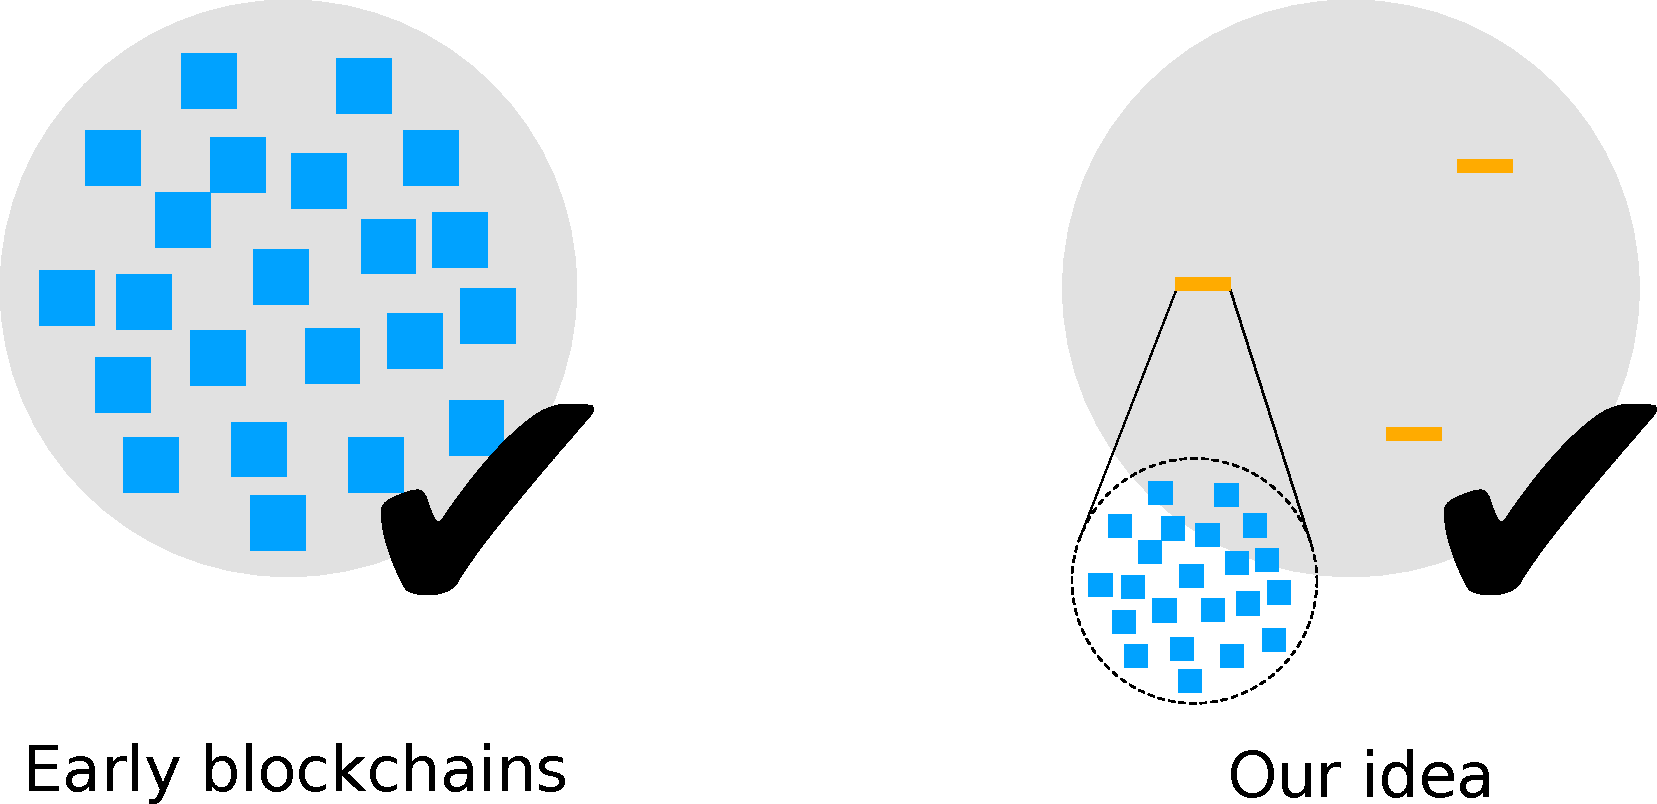
\includegraphics[width=0.7\textwidth]{idea}
  \centering
  \end{figure}
\end{frame}

\subsection{System model}
\subsection{Architecture overview}
\begin{frame}{\subsecname}
  \begin{center}
  {\Large The four components of \textsc{Checo}\footnote{\textsc{Che}ckpoint \textsc{co}nsensus}} 
  \begin{figure}[h]
  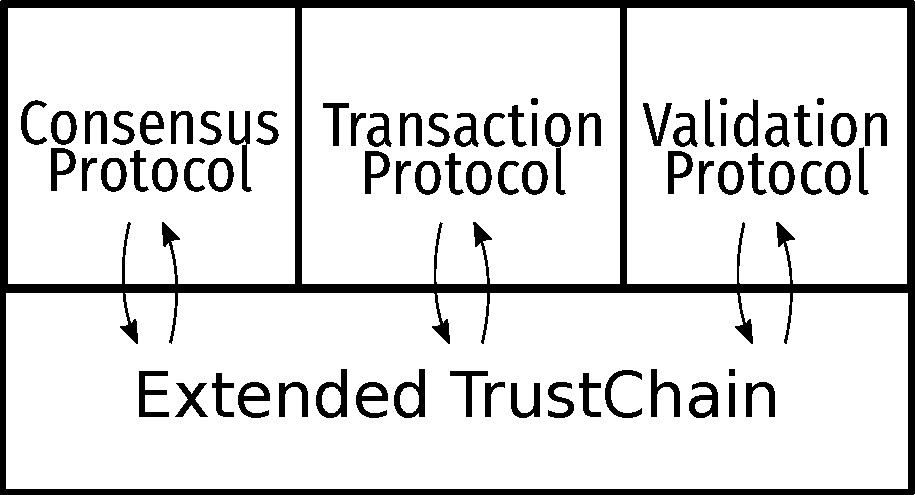
\includegraphics[width=0.7\textwidth]{architecture-wo-title}
  \centering
  \end{figure}
  \end{center}
  \note{
    \begin{itemize}
    \item The primary data structure is the Extended TrustChain, extension of our prior work
    \item The three protocols the tasks as their name suggests
    \item They are independent and run concurrently
    \item The only synchronisation happens via the Extended TrustChain
    \item But in no part of those protocol do we lock the Extended TrustChain
    \end{itemize}
  }
\end{frame}

\subsection{Extended TrustChain}
\begin{frame}{\subsecname}
  \begin{figure}[h]
  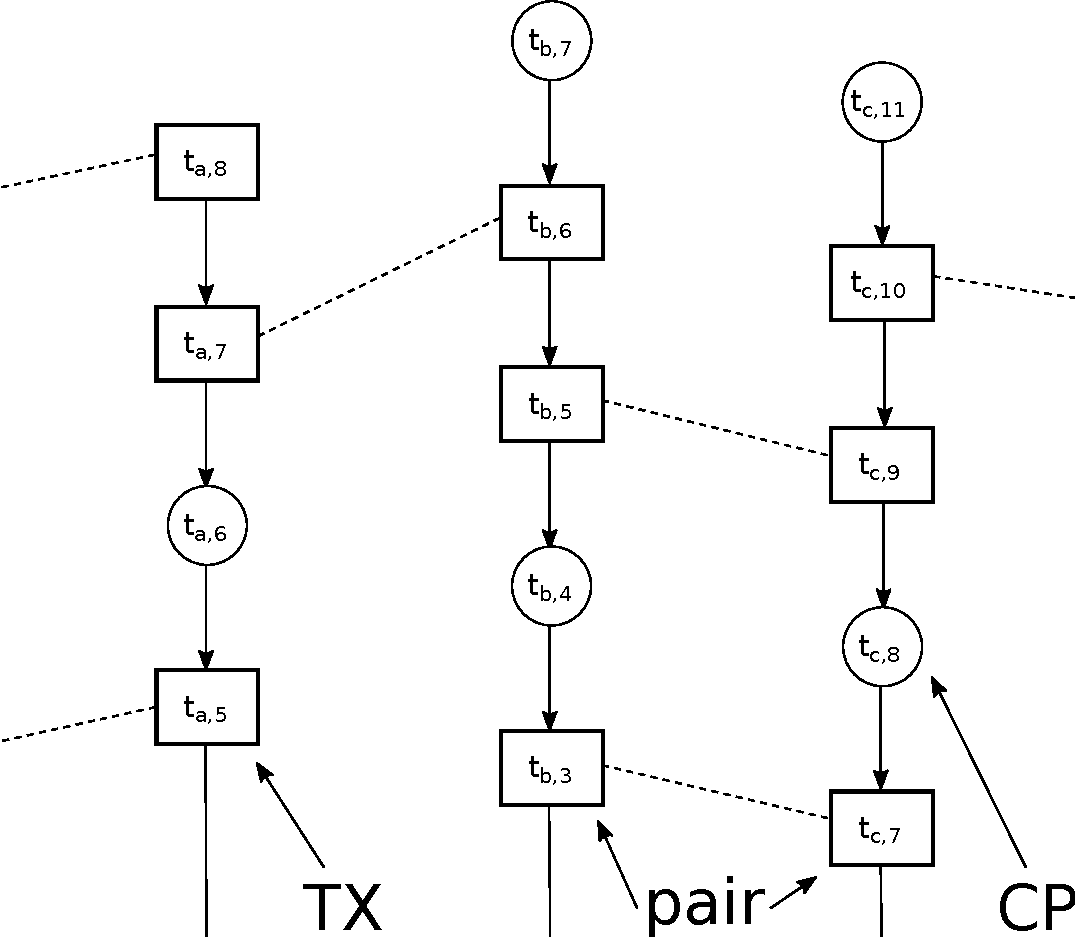
\includegraphics[width=0.84\textwidth]{trustchain-good-cp}
  \centering
  \end{figure}
  \note{
    \begin{itemize}
      \item In this example there are three nodes
      \item Each node maintains their personal hash chain and genesis block
      \item Squares are TX blocks and circles are CP blocks
      \item Explain the block content in caption
      \item The dotted line represent pairs of TX blocks
      \item Geared with the understanding of our data structure, we are ready to talk about the consensus protocol
    \end{itemize}
  }
\end{frame}

\begin{frame}{\subsecname:~Transaction (TX) block}
\begin{itemize}
  \item Goal: record transactions
  \item A transaction is an agreement on a piece of data, i.e. digitally signed by both parties
  \item It is represented by a pair of TX blocks
\end{itemize}
\begin{figure}[h]
  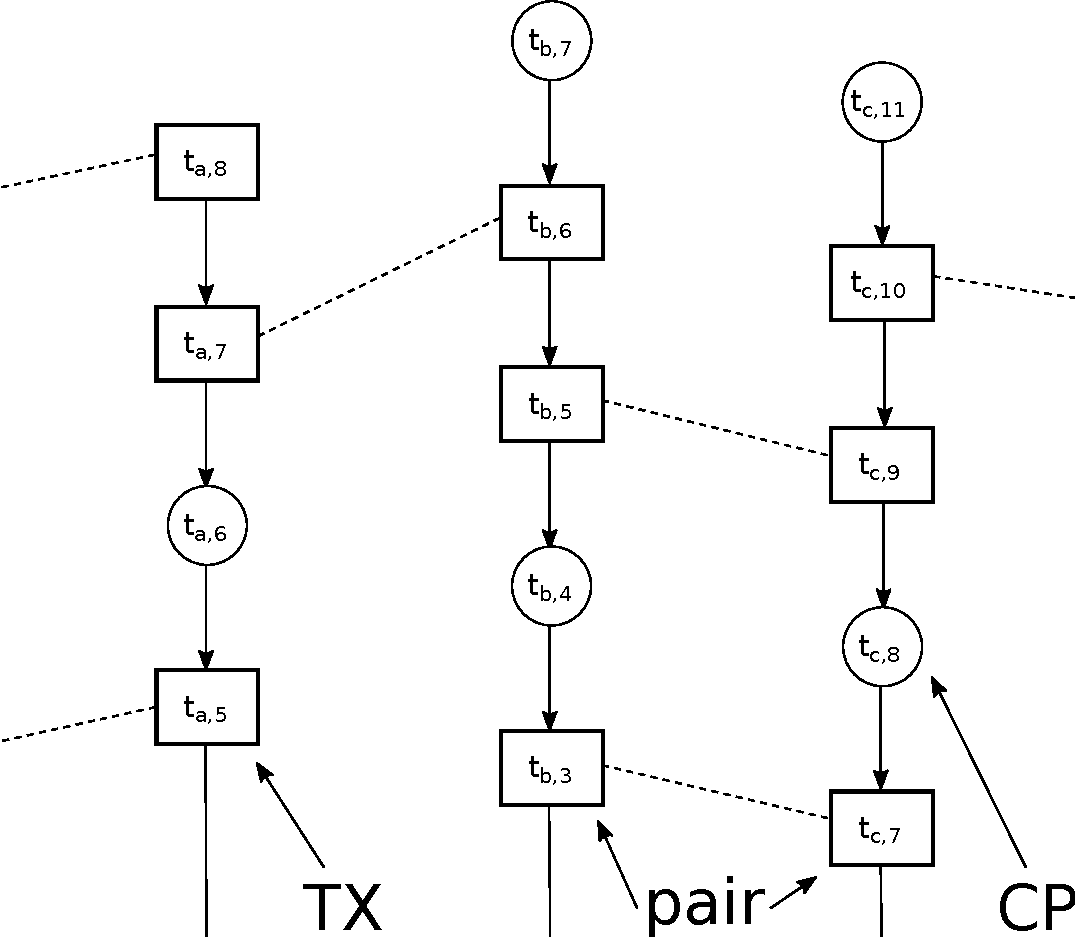
\includegraphics[trim={7cm 8.2cm 2cm 2.55cm},clip,width=0.7\textwidth]{trustchain-good-cp}
  \centering
\end{figure}
\end{frame}

\begin{frame}{\subsecname:~Checkpoint (CP) block}
  \begin{itemize}
    \item Goal: represent the state of the chain using a single digest
    \item A collection of CP blocks from all the nodes represent the state of the system
    \item Nodes become aware of the system state by running our consensus protocol
  \end{itemize}
\begin{figure}[h]
  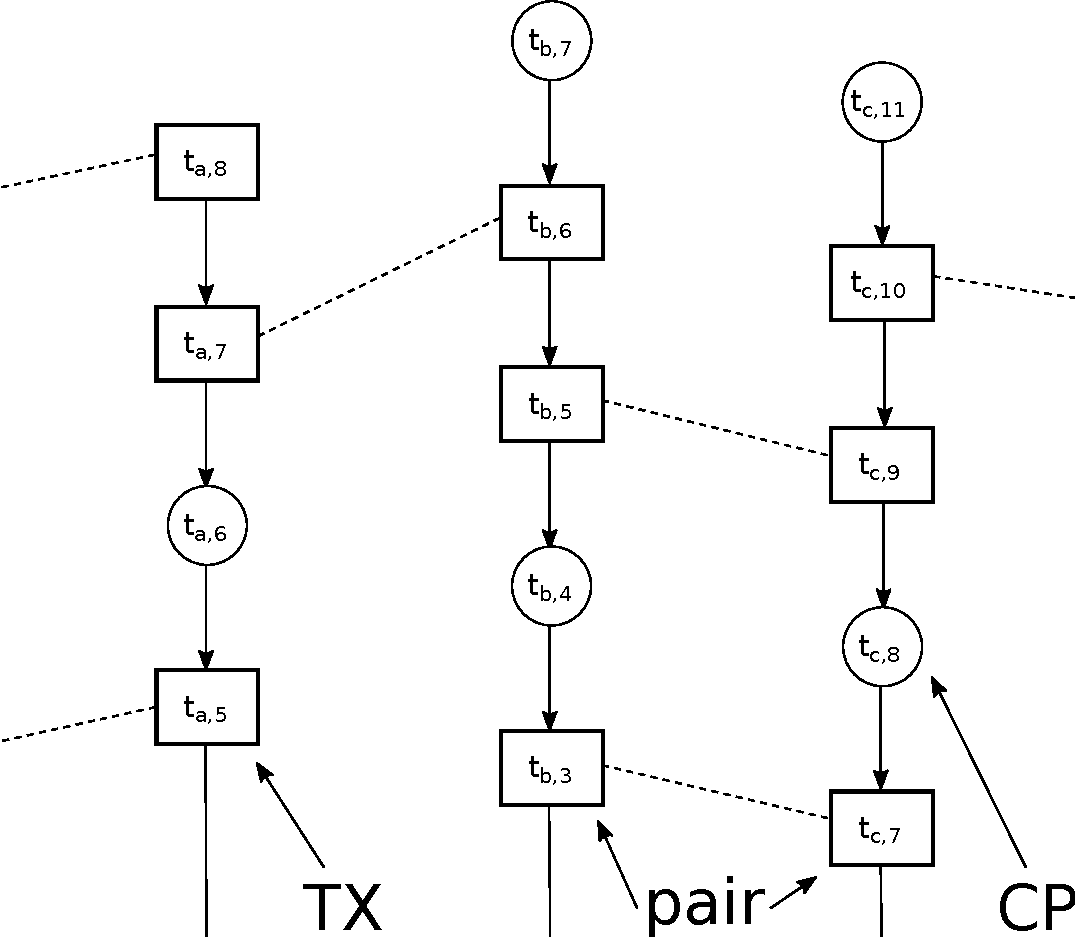
\includegraphics[trim={7cm 2.505cm 2cm 8.55cm},clip,width=0.7\textwidth]{trustchain-good-cp}
  \centering
\end{figure}
\end{frame}

\begin{frame}{\subsecname:~Fragment of a TX block}
  \begin{figure}[h]
  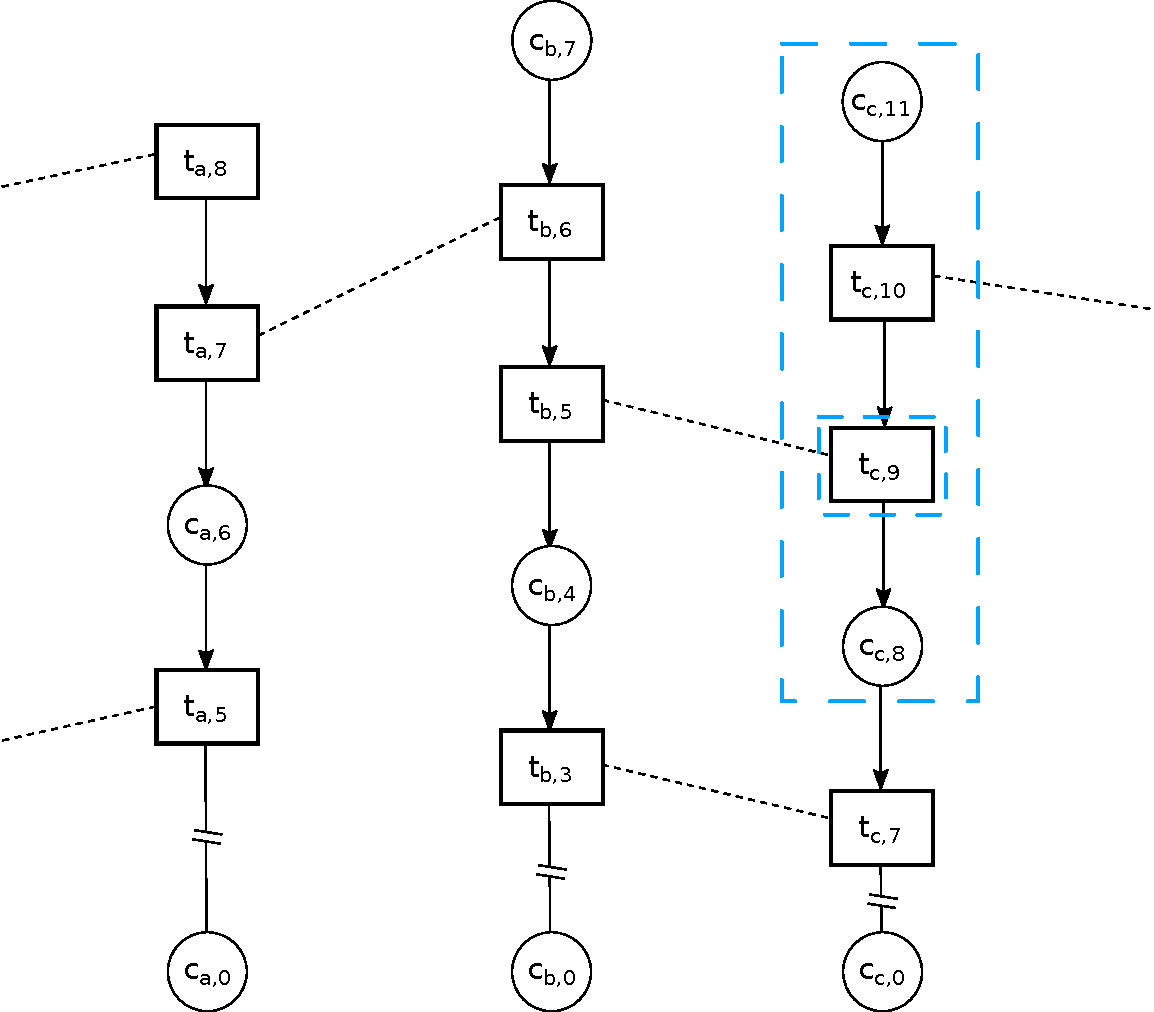
\includegraphics[width=0.84\textwidth]{trustchain-good-cp-frag}
  \centering
  \end{figure}
\end{frame}

\subsection{Consensus protocol}

\begin{frame}{\subsecname}
  \begin{itemize}
    \item Goal 1: reach consensus on a collection of CP blocks amongst all the nodes
    \item Goal 2: create new CP blocks at the end of the protocol
    \item Uses an existing fault-tolerant consensus algorithm (HoneyBadgerBFT\footnote{MXCSS, CCS16}) as the building block
    \item But it cannot be used in a large network due to high communication complexity
    \item We overcome this limitation by selecting a small number of \emph{facilitators} from the network to run HoneyBadgerBFT
  \end{itemize}
\end{frame}

\begin{frame}{\subsecname}
  \begin{figure}
    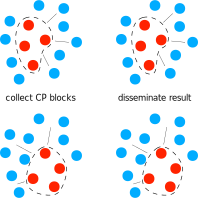
\includegraphics[width=1.0\textwidth]{consensus-overview}
    \centering
  \end{figure}
\end{frame}

\subsection{Transaction protocol}
\begin{frame}{\subsecname}
  \begin{figure}[h]
  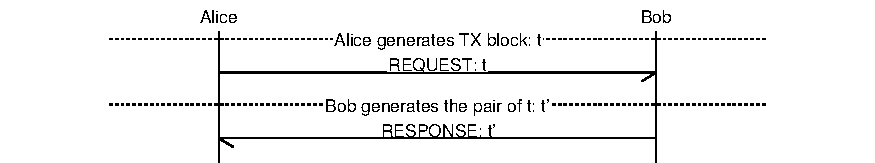
\includegraphics[width=1.0\textwidth]{tx-proto}
  \centering
  \end{figure}
\begin{itemize}
\item Two TX blocks are generated on the chains of Alice and Bob
\item No guarantee that nodes follow this protocol
\item Contrary to early blockchain systems, we do not broadcast transactions
\end{itemize}
\end{frame}

\subsection{Validation protocol}
\begin{frame}{\subsecname}
  \begin{figure}[h]
  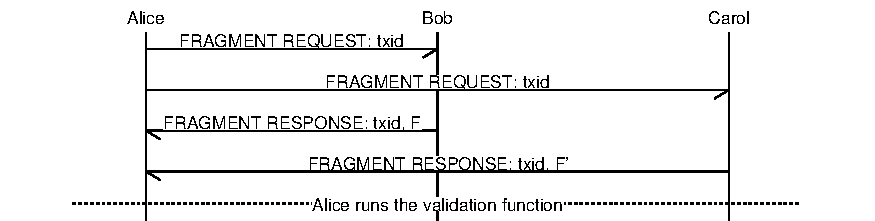
\includegraphics[width=1.0\textwidth]{vd-proto}
  \centering
  \end{figure}
\begin{itemize}
\item To check that the transaction protocol is correctly followed
\item Alice needs the fragment of the TX on Bob's hash chain 
\item Validation function checks whether the fragment is OK and contain the transaction
\item Can be generalised---any node may run the validation protocol on any transaction (does not need to be their own)
\end{itemize}
\end{frame}

\begin{frame}{\subsecname:~properties}
\emph{Consensus on CP blocks $\rightarrow$ consensus on transactions}
\bigskip
\begin{itemize}
  \item CP blocks of the fragments are ``anchored'' due to the consensus protocol
  \item It is difficult to modify the fragment once ``anchored''
  \item Since the transaction protocol and the validation protocol only use point-to-point communication,
  we achieve horizontal scalability.
\end{itemize}
\end{frame}

\section{Experimental results}
\begin{frame}{Implementation and experiment setup}
  \begin{itemize}
    \item Free and open source implementation on Github:
      \url{https://github.com/kc1212/checo}
    \item SHA256 for hash functions and Ed25519 for digital signature
    \item Experiment on the DAS-5\footnote{\url{http://www.cs.vu.nl/das5/}}
    \item Up to 1200 nodes
    \item A third of the facilitators are malicious
  \end{itemize}
\end{frame}

\begin{frame}{Validated transaction throughput (random node)}
  \begin{figure}[h]
  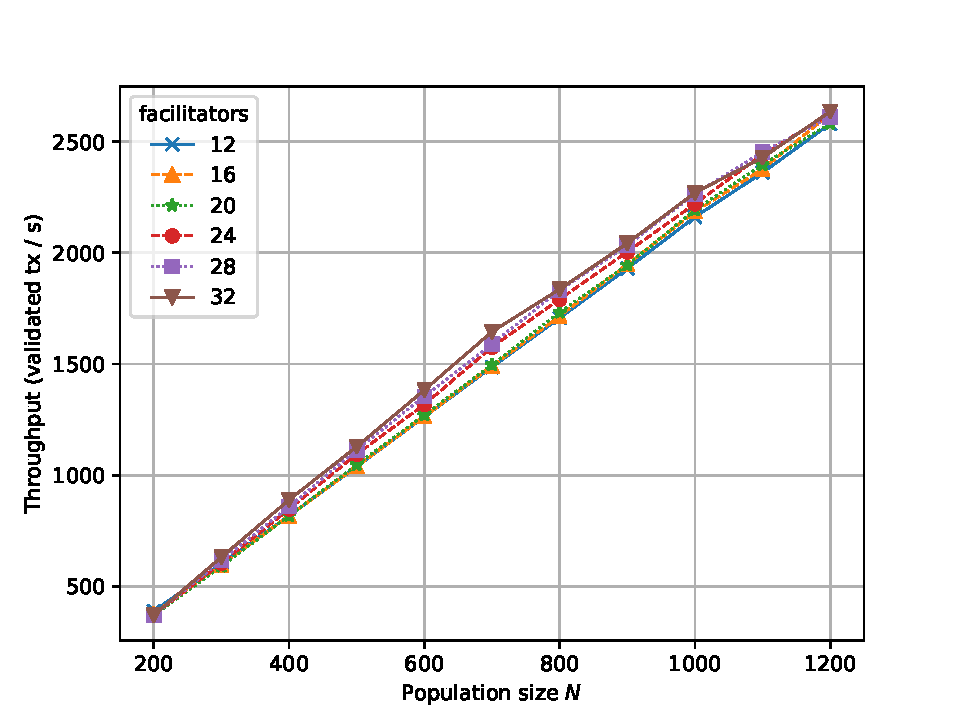
\includegraphics[width=0.95\textwidth]{neighbour-random/throughput-vs-population}
  \centering
  \end{figure}
\end{frame}

\begin{frame}{Validated transaction throughput (fixed neighbour)}
  \begin{figure}[h]
  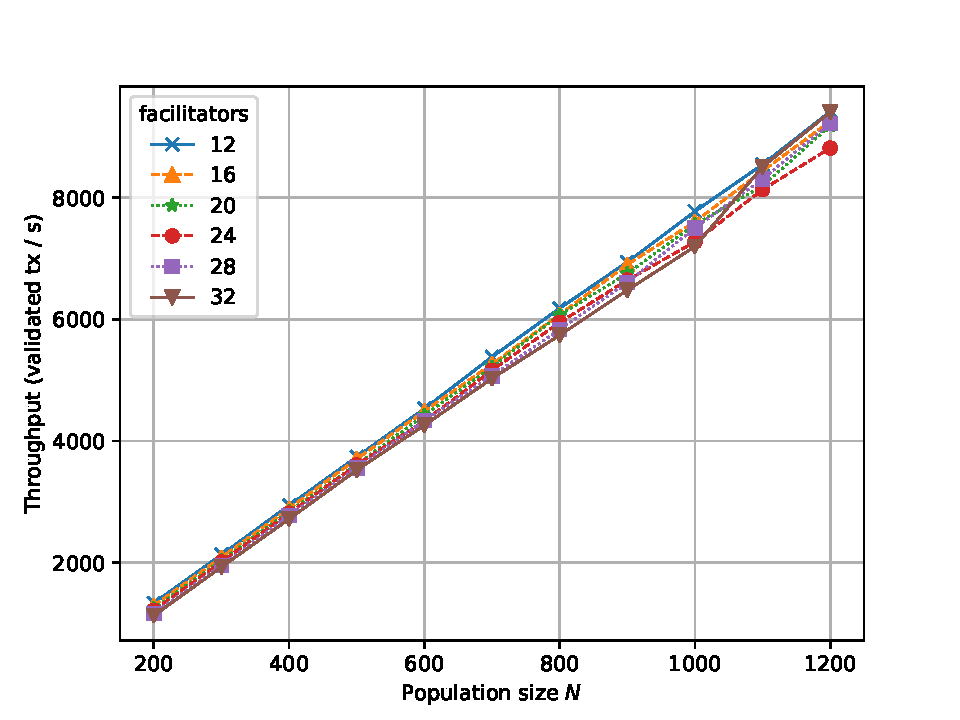
\includegraphics[width=0.95\textwidth]{neighbour-fixed/throughput-vs-population}
  \centering
  \end{figure}
\note{No need to request for fragment every time a TX needs to be validated. Upon receiving a fragment, validate as many TX as possible.}
\end{frame}

\section{Conclusion}
\begin{frame}{\secname}
    Our contribution:
  \begin{itemize}
      \item We design a blockchain consensus protocol---\textsc{Checo} with horizontal scalability
      \item We formally analyse CHECO to ensure correctness
      \item Our experimental evaluation show strong evidence of our claim.
  \end{itemize}
      Future perspective:
  \begin{itemize}
      \item Improve fault-tolerance using ByzCoinX from OmniLedger
      \item Design and evaluate UTXO-style transactions (new paper to appear in Crypto Valley Conference)
      \item Assume a permissionless model
  \end{itemize}
\end{frame}

% \begin{frame}{Bibliography}
% \printbibliography
% \end{frame}

\section*{Extras}
\begin{frame}[noframenumbering]{TX block}
  \begin{enumerate}
    \item Hash pointer to the previous block
    \item Sequence number
    \item Transaction ID
    \item Public key of the counterparty
    \item Transaction message $m$
    \item Signature the five items above
  \end{enumerate}
  \vfill
  A transaction is represented by a \emph{pair} of TX blocks
\end{frame}

\begin{frame}[noframenumbering]{CP block}
  \begin{enumerate}
    \item Hash pointer to the previous block
    \item Sequence number
    \item Digest of consensus result, i.e.~a set of CP blocks
    \item Round number $r$
    \item Signature on the four items above
  \end{enumerate}
\end{frame}

\begin{frame}[noframenumbering]{Background on ACS}
  \begin{itemize}
    \item Asynchronous common subset
    \item A simplification of HoneyBadgerBFT
    \item $n$ nodes
    \item $t$ nodes may be malicious
    \item Input: every node proposes a set of values, e.g., $\{A, B\}, \{B, C\}, \dots$
    \item Output: set union of the majority, e.g., $\{A, B, C, \dots \}$
  \end{itemize}
\end{frame}

\subsection*{Consensus protocol}
\begin{frame}[noframenumbering]{\subsecname:~part 1}
  \begin{figure}[h]
  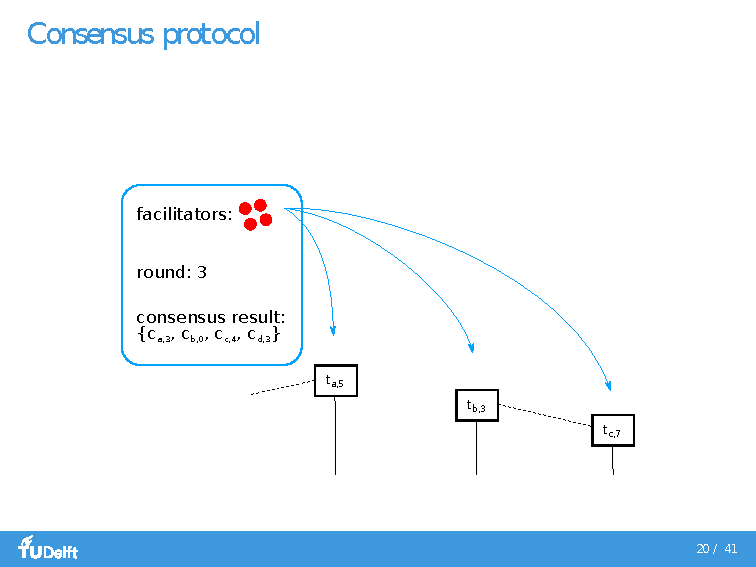
\includegraphics[trim={2cm 1.5cm 2cm 1.5cm},clip,width=0.75\textwidth]{trustchain-1}
  \centering
  \end{figure}
  \note{Suppose we are in a state where $\C_{r - 1}$ has just been agreed by some facilitators but not yet propagated.}
\end{frame}

\begin{frame}[noframenumbering]{\subsecname:~part 2}
  \begin{figure}[h]
  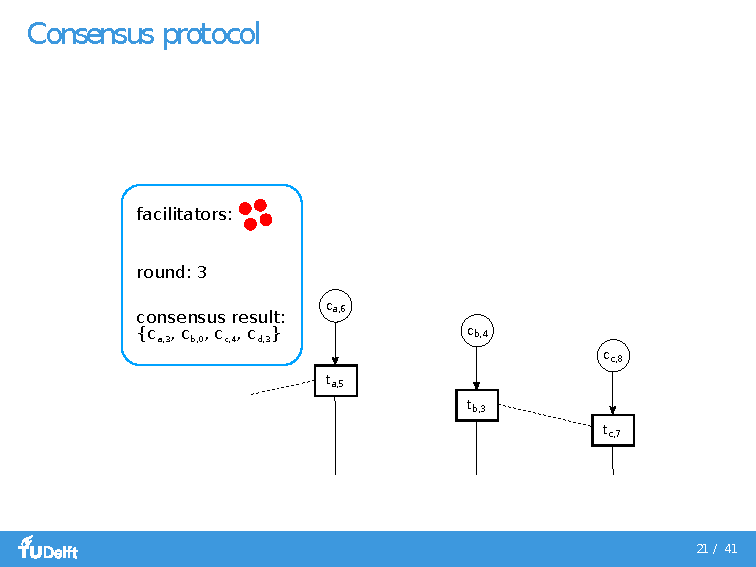
\includegraphics[trim={2cm 1.5cm 2cm 1.5cm},clip,width=0.75\textwidth]{trustchain-2}
  \centering
  \end{figure}
  \note{Nodes receive consensus result $\C_{r - 1}$,
    first $n$ nodes ordered by $\textsf{H}(\C_{r-1} || pk)$ become $\F_{r-1}$,
    send the new CP blocks to $\F_{r-1}$.}
\end{frame}

\begin{frame}[noframenumbering]{\subsecname:~part 3}
  \begin{figure}[h]
  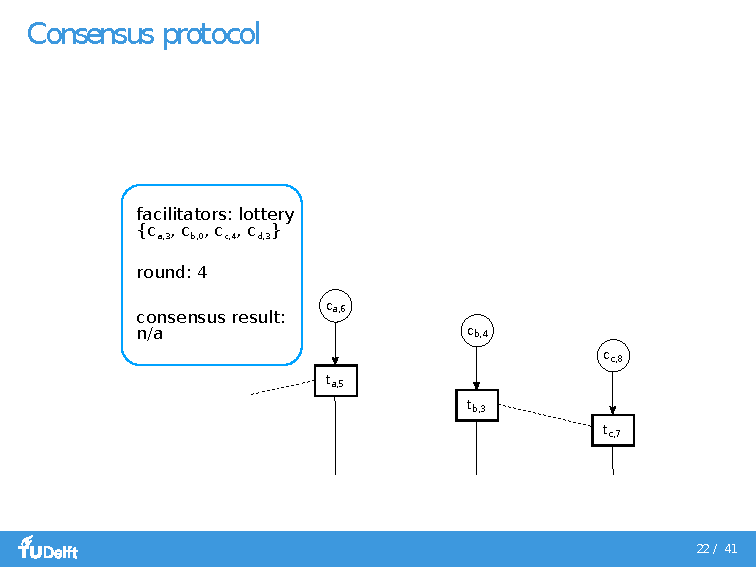
\includegraphics[trim={2cm 1.5cm 2cm 1.5cm},clip,width=0.75\textwidth]{trustchain-3}
  \centering
  \end{figure}
\end{frame}

\begin{frame}[noframenumbering]{\subsecname:~part 4}
  \begin{figure}[h]
  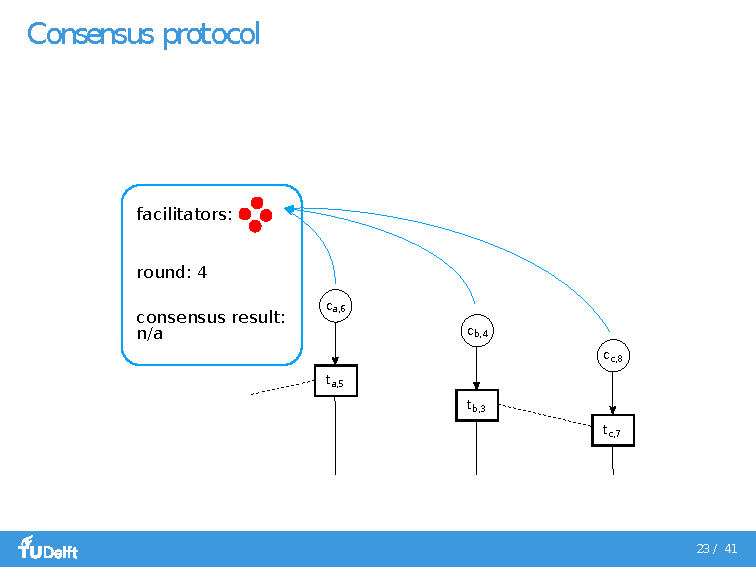
\includegraphics[trim={2cm 1.5cm 2cm 1.5cm},clip,width=0.75\textwidth]{trustchain-4}
  \centering
  \end{figure}
\end{frame}

\begin{frame}[noframenumbering]{\subsecname:~part 5}
  \begin{figure}[h]
  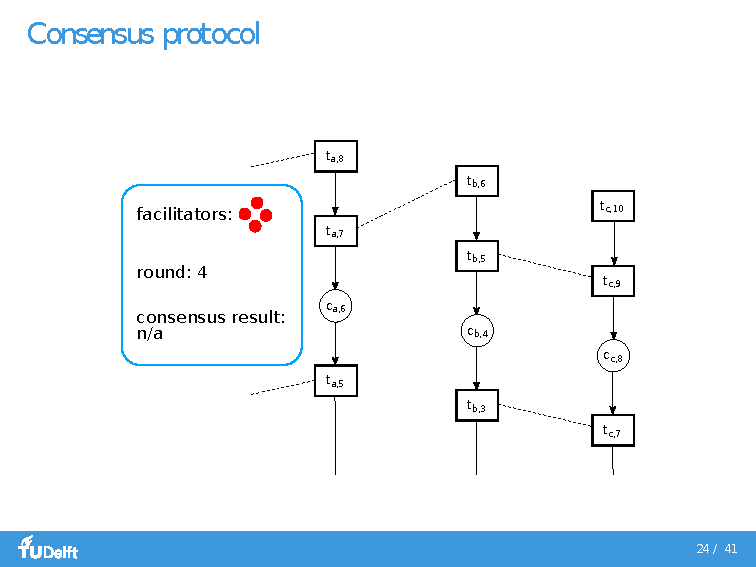
\includegraphics[trim={2cm 1.5cm 2cm 1.5cm},clip,width=0.75\textwidth]{trustchain-5}
  \centering
  \end{figure}
  \note{Transactions carry on as usual in round $r$,
  while facilitators are trying to reach consensus on the new CP blocks concurrently.}
\end{frame}

\begin{frame}[noframenumbering]{\subsecname:~part 6}
  \begin{figure}[h]
  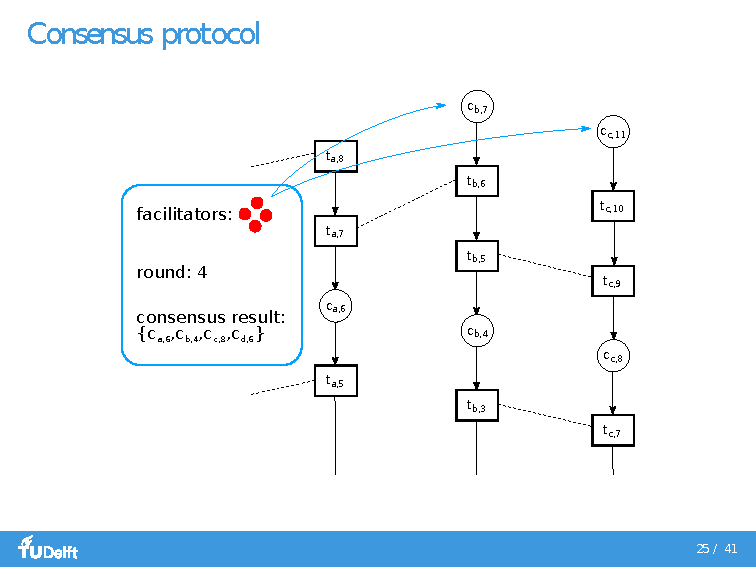
\includegraphics[trim={2cm 1.5cm 2cm 1.5cm},clip,width=0.75\textwidth]{trustchain-6}
  \centering
  \end{figure}
  \note{$\F_{r-1}$ agree and disseminate $\C_r$,
  CP blocks at round $r-1$ ($c_{a, 6}, c_{b, 4}, c_{c,8}$) should be in $\C_r$.}
\end{frame}

\begin{frame}[noframenumbering]{Effect of the number of facilitators (fixed neighbours)}
  \begin{figure}
    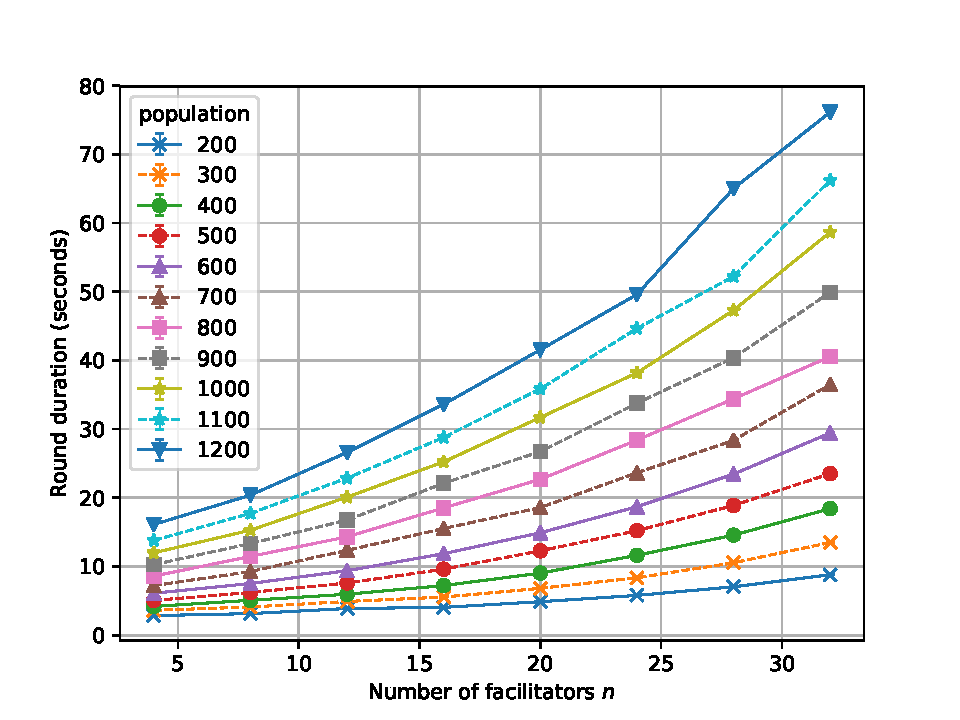
\includegraphics[width=0.9\textwidth]{neighbour-fixed/round-duration-vs-facilitators}
    \centering
  \end{figure}
\end{frame}

\begin{frame}[noframenumbering]{Effect of the number of facilitators (random neighbours)}
  \begin{figure}
    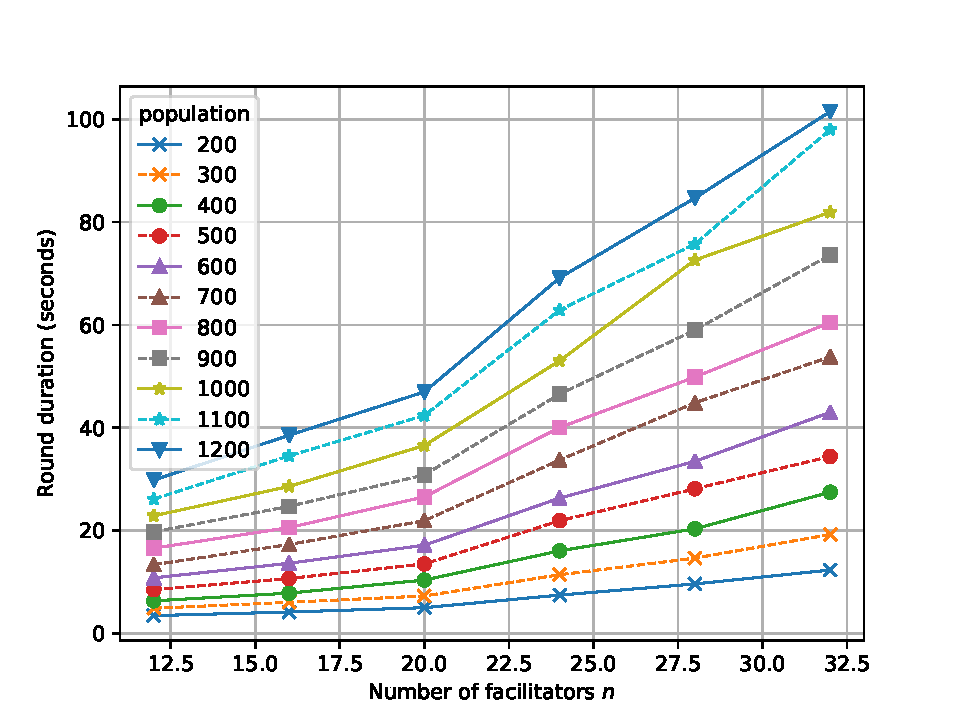
\includegraphics[width=0.9\textwidth]{neighbour-random/round-duration-vs-facilitators}
    \centering
  \end{figure}
\end{frame}

\begin{frame}[noframenumbering]{Stress test (fixed neighbour)}
  \begin{figure}[h]
  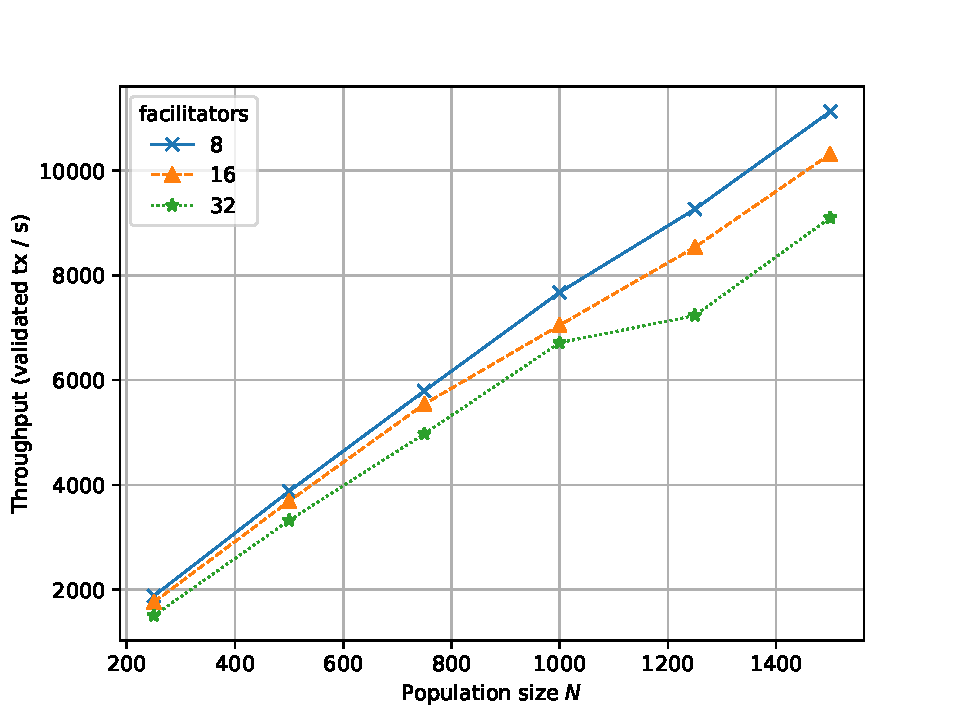
\includegraphics[width=0.9\textwidth]{throughput-vs-population-large}
  \centering
  \end{figure}
\end{frame}


\end{document}


% Sybils
% facilitator set?
% incentivise?
% attack (predict) of facilitator
% appoint facilitator
% liveness / non-responsive / slow
% drawbacks
% 
